\renewcommand{\LangOO}{\ensuremath{{\mathcal{L}}_{ul}}\xspace }

\section{The underlying programming language \LangOO}  
\label{sect:underlying}

\subsection{\LangOO syntax and runtime configurations}
\label{sub:Loo} 
{This work} is based on \LangOO, a {small}, imperative, sequential,  class based, typed, object-oriented language. 
 {We believe, however, that the work can easily be adapted to any capability safe language with some form of encapsulation. 
Wrt to encapsulation and  capability safety},  \LangOO supports private fields, private and public methods, unforgeable addresses, and no ambient authority (no static methods, no address manipulation).
 It has a simple concept of module with module-private fields and methods, described in Sect. \ref{sect:execution}.
 The definition of \LangOO~ {can be found in   {Appendix \ref{app:loo}.}\footnote{{{The examples in this paper are using  a slightly richer syntax for greater readability.}}}.
 
A \LangOO state, $\sigma$,  consists of a  heap $\chi$, and a   stack. 
{A stack  is a sequence of frames, $\phi_1\!\cdot\!...\!\cdot\! \phi_n$.}
A  frame, $\phi$, consists of a local variable map and a continuation, \ie a sequence of statements to be executed.
The top frame in a state $(\phi_1\!\cdot\!...\!\cdot\! \phi_n, \chi)$ is $\phi_n$. 


 
\paragraph{Notation} We adopt the following unsurprising notation:
\label{s:notation}
\begin{itemize}
\item
{An object is uniquely identified by the address that points to it. We shall be talking of objects $o$, $o'$ when talking less formally, and of addresses, $\alpha$, $\alpha'$, $\alpha_1$, ...  when more formal.}
\item
$x$, $x'$, $y$, $z$, $u$, $v$, $\va$  are \sdN{variables}. 
% I have removed atoms; we either have addresses of variable
% $\va$, $\va'$ ... are either addresses or variables. %, we call these \emph{\atoms}.
\item
$\alpha \in \sigma$ means that $\alpha$ is defined in the heap of $\sigma$, and $x\in \sigma$ means that $x$ is defined in the top frame of $\sigma$.
Conversely,  $\alpha\notin\sigma$ and $x\notin\sigma$ %, and $\va \notin A$ h
 have the obvious meanings.
$\interpret{\sigma}{\alpha}$  is $\alpha$; and $\interpret{\sigma}{x}$  is the value to which  $x$  is mapped in the top-most frame of $\sigma$'s stack, 
and $\interpret{\sigma}{e.f}$ looks up in $\sigma$'s heap the value of $f$ for the object  $\interpret{\sigma}{e}$.
% too much detail?
% Note that $\interpret{\sigma}{e}$ is not defined when $e$ contains a method call or a ghost field.
\item %The  update
$\phi[x \mapsto \alpha]$ updates  the variable map  of $\phi$,  
and  $\sigma[x \mapsto \alpha]$ updates the top frame of $\sigma$.
\item
$A[e/x]$ is textual substitution where we replace all occurrences of $x$ in $A$ by $e.$ 
\item
As usual, $\overline q$ stands for  sequence $q_1$, ... $q_n$, where $q$ can be an address, a variable,    a frame, an update or a substitution.
Thus,   $\sigma[\overline{x \mapsto \alpha}]$ and $A[ \overline{e/y}]$ 
% applies the substitutions $\overline{x \mapsto \alpha}$ to the top frame.
have the expected meaning.
\item
$\phi.\prg{cont}$ is the continuation of frame $\phi$, and  $\sigma.\prg{cont}$ is the continuation in the top frame.
\item
$text_1 \txteq text_2$ expresses that $text_1$ and $text_2$ are textually equal.
% the below moved to appendix
%  $s_1 \txtin   s_2$  means  $s_1 \txteq  s_2$ or  $s_2 \txteq  s_1; s_3$ for some $s_3$, where $s_1$, $s_2$, and $s_3$ are program statements. 
\item
We define the depth of a stack as $\DepthFs {\phi_1...\phi_n} \triangleq n$, For states, $\DepthSt {(\overline \phi, \chi)} \triangleq  \DepthFs {\overline \phi}$.
The  operator $\RestictTo  \sigma k$ truncates the stack up to the $k$-th frame: % from $\sigma$. Namely, 
 $\RestictTo {(\phi_1...\phi_k...\phi_n,\chi)} {k}  \triangleq   (\phi_1...\phi_k,\chi)$
\item
{ $\vs(stmt)$ returns the variables which appear in $stmt$. For example, $\vs(u:=y.f)$=$\{u,y\}$.}
\end{itemize}

  

  
\subsection{\LangOO Execution}
\label{sect:execution}

 \LangOO execution is described by a small steps operational semantics of the shape $\leadstoOrig  {\Mtwo} {\sigma}   {\sigma'}$ 
 -- {\cf Fig. \ref{f:evaluation}.} 
  $\Mtwo$ stands for one or more modules, where a
  module,  $M$, maps class names to class definitions. 
{The semantics enforces dynamically a simple form of module-wide privacy: 
Fields may be read or written only if the class of the object whose field is being read or written, and the class of the object which is reading or writing belong to the same module.}
Private methods may be called only if the class of the receiver (the object whose method is being called), and the class of the caller (the object which is calling) belong to the same module.
Public methods may always be called.

The semantics is unsurprising :  
In $\sigma$, the  top frame's continuation contains the statement to be  executed next.  
 Statements may assign to variables, allocate new objects, 
perform field reads and writes on objects, and
 call methods on those objects. 
When a method is called, a new frame is pushed onto the stack; this frame  maps \prg{this} and the formal parameters to  the values for the receiver and other arguments, and the continuation to the body of the method. 
{Methods are expected to store their return values in the variable \prg{res}.}
 When the continuation is {empty ($\epsilon$), the frame is popped and the value of \prg{res}
 {\susan{\footnote{\prg{res} is implicit like \prg{this}}}}
 from the popped frame  is stored  in the variable map of the top frame.}
%In other aspects, the semantics is unsurprisring.%we return from that call, its frame is  popped, and execution continues in the context of the calling method. 
%The relation $\leadstoOrigStar  {\Mtwo} {\_}   {\_}$  is the reflexive, transitive closure of $\leadstoOrig  {\Mtwo} {\_}   {\_}$ .
Wlog, \sdN{to simplify some proofs} we  require, as in Kotlin, that method bodies do not assign to formal parameters, , \cf Def.  \ref{def:wf:state}.  
%This simplifies some proofs and gives rise to a well-formedness requirement for states, 
%$\models \sigma$, which guarantees that for all frames  on the stack, the actual parameters of a method call in a  caller frame have the same values as the formal parameters in the called frame, \cf Def.  \ref{def:wf:state}. 
%From now on we require implicitly that $\models \sigma$.

Fig. \ref{fig:UpSemantics} illustrates  such  ${\leadstoN}$ executions, where we distinguish
  steps within the same  call ($\rightarrow$),\   entering a method  ($\uparrow$),\    returning from a method  ($\downarrow$).
Thus,  $\sigma_8 \rightarrow \sigma_9$ indicates that  $\leadstoOrig {\Mtwo}{\sigma_8}   {\sigma_9} $ is a step within the same call, 
\ $\sigma_9 \uparrow \sigma_{10}$ indicates that $\leadstoOrig {\Mtwo}{\sigma_9}   {\sigma_{10}} $ is a method entry, \ with 
  $\sigma_{12} \downarrow \sigma_{13}$   the corresponding return. 
In general,  $\leadstoOrigStar  {\Mtwo} {\sigma}   {\sigma'}$ may involve  any number of  calls or returns: \eg
 $\leadstoOrigStar  {\Mtwo} {\sigma_8}   {\sigma_{12}}$ involves one call and no return,
while $\leadstoOrigStar  {\Mtwo} {\sigma_{10}}   {\sigma_{15}}$,   involves no calls and two returns.


\begin{figure}[htb]
\begin{tabular}{|c|}
 \hline %  \\ -- this added one vertical space
\resizebox{7cm}{!}{
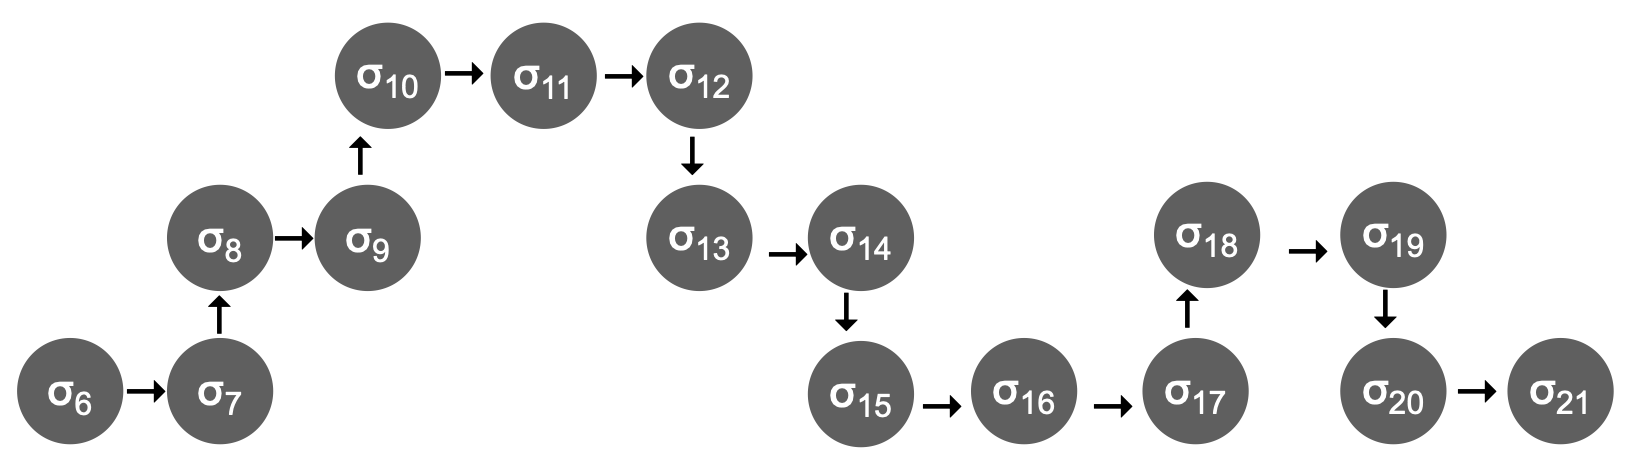
\includegraphics[width=\linewidth]{diagrams/bounded2.png}
} 
 \\
\hline

\end{tabular}
   \caption{$\rightarrow$:\  step within the same method; \ \ $\uparrow$:\    entering a method;\ \  $\downarrow$:  returning from a method}
   \label{fig:UpSemantics}
 \end{figure}
 

\section{\susan{Fundamental} Concepts}
\label{s:auxiliary}

{The semantics of our assertion language % , \AssertLang, 
is based on three concepts built on} \LangOO: {method calls and returns, scoped execution}, and locally reachable objects.}

\subsection{ Method Calls and Returns}
 
Method calls and returns are \susan{critical} for our work. 
They are characterized through pushing/popping   frames on the stack.  
The operator   $ \PushS  {\phi} {\sigma}$ pushes 
frame $\phi$ onto the stack of $\sigma$,
 \susan{ while
 operator $\sigma$ $\popSymbol$   pops a frame of $\sigma$'s stack and updates the continuation and variable map.}

 
 
\forget{
\begin{definition}
\label{def:push:frame}
Given a state $\sigma$, addresses $\overline \alpha$, a frame $\phi$,  variables or addresses $\overline \va$, we define
\begin{itemize}
\item
 $ \PushSF  {\phi} {\sigma} \ \triangleq \ ({\overline{\phi}\cdot\phi}, \chi)$ \ \ \  if \ \ \  $\sigma=(\overline{\phi}, \chi)$.
%\item
%$ \PushS  {\alpha} {\sigma} \ \triangleq\ \{ \ \sigma' \ \mid\ \exists \phi  \ s.t.\ \ 
%   \sigma'=\PushSF  {\phi} {\sigma}  \ \wedge\    Rng(\phi)=\overline \alpha \ \   \ \}$
%\item
%{$ \PushS  {\va}  {\sigma}\  \triangleq\     \PushS  {\interpret {\sigma} {\va}} {\sigma} $.}
\item
$ \ \sigma\, \popSymbol \ \ \  \triangleq\   { (\overline{\phi}\cdot (\phi_n[\prg{cont}\mapsto stmt][x \mapsto \interpret {\phi_n}{ret}]), \chi)}$ \ \ \  if \\
 $\strut \hspace{1.2cm}  \exists x, y_0, \overline y. [ \ \sigma=(\overline{\phi}\cdot\phi_n\cdot\phi_{n+1}, \chi)$, and $\phi_n(\prg{cont})\txteq x:= y_0.m(\overline y); stmt \ ]$
\end{itemize}
 \end{definition}}
%\footnoteSD{\red{DO we also need that $\overline \alpha$ were locally reachable in $\sigma$?}}
\begin{definition}
\label{def:push:frame}
Given a state $\sigma$, and a frame $\phi$,  we define
\begin{itemize}
\item
 $ \PushSF  {\phi} {\sigma} \ \triangleq \ ({\overline{\phi}\cdot\phi}, \chi)$ \ \ \  if \ \ \  $\sigma=(\overline{\phi}, \chi)$.
\item
$ \ \sigma\, \popSymbol \ \ \  \triangleq\   { (\overline{\phi}\cdot (\phi_n[\prg{cont}\mapsto stmt][x \mapsto \interpret {\phi_n}{\prg{res}}]), \chi)}$ \ \ \  if \\
 $\strut \hspace{1.5cm} \sigma=(\overline{\phi}\cdot\phi_n\cdot\phi_{n+1}, \chi)$, and $\phi_n(\prg{cont})\txteq x:= y_0.m(\overline y); stmt $
\end{itemize}
 \end{definition}

Consider Fig. \ref{fig:UpSemantics} again: $\sigma_8 = \PushSF  {\phi} {\sigma_7}$ for some $\phi$, and  $\sigma_{15}$=$\sigma_{14} \popSymbol$
--  thus $\sigma_8$ is a {\emph{called}} state for 
 $\sigma_7$, and  $\sigma_{15}$ is the {\emph{return}} state from 
 $\sigma_{14}$.
% Note that $\sigma = \sigma' \popSymbol$ iff $\sigma'\!\in\!\PushS  {\phi} {\sigma}$; we can see that 
% Also, 
% $\sigma_{14}\!\in\!\PushS  {\phi'} {\sigma_{15}}$ for some $\overline {\alpha'}$ -- {thus $\sigma_{15}$ is a caller state for  $\sigma_{14}$}.
%\footnote{$\phi'$ may differ from $\phi$, because between $\sigma_8$ and $\sigma_{15}$ there may 
% have been assignments to local variables.} 

 
 \subsection{Scoped Execution}
 \label{sect:bounded}

\sdN{\emph{Scoped invariants}, \cf \S  \ref{sect:approach:scoped},}  ensure that if a state $\sigma$ satisfies $A$, then all future states reachable from $\sigma$—including nested method calls and returns but \forget{excluding}{\emph{stopping} before}  the return from the active call in $\sigma$—will also satisfy $A$. For example, let $\sigma$ make an external call, transitioning to $\sigma_1$,    execution of $\sigma_1$'s continuation results in $\sigma_2$, and $\sigma_2$ returns  to $\sigma'$. 
Suppose the module guarantees $\TwoStatesN {\overline{x}} {A}$, and $\sigma \not\models A$, but $\sigma_1 \models A$. 
\sd{Scoped invariants %require   
\se{ensure} $\sigma_2 \models A$, but allow   $\sigma' \not\models A$.}
\sue{Although similar to scoped invariants, neither history invariants nor object invariants provide the functionality we need.}

\sdN{\emph{History  invariants}} \cite{liskov94behavioral,usinghistory,Cohen10}, instead, allow future states to contain the return from the active call, and thus, \sdN{would  require that   $\sigma' \models A$. Thus, they are,}  for our purposes,  both
 \emph{unenforceable} and overly \emph{restrictive}.\ \  \emph{Unenforceable}: \ Take $A \txteq \inside{a.\prg{key}}$,  assume  in $\sigma$ a path to an external object which has access to $a.\prg{key}$, assume that path is unknown in $\sigma_1$: then, the transition from $\sigma_1$ to $\sigma_2$ cannot eliminate that path—hence, $\sigma' \not\models \inside{a.\prg{key}}$.\ \  \emph{Restrictive}:\ Take $A \txteq \inside{a.\prg{key}}\wedge a.\prg{blnce}\geq b$; then,  requiring  $A$   to hold in all states from $\sigma_1$ until termination would prevent all future withdrawals from $a$, rendering the account useless.

\sdN{\emph{Object}} invariants  \cite{Meyer92,MeyerDBC92,BarDelFahLeiSch04,objInvars,MuellerPoetzsch-HeffterLeavens06}, on the other hand, require the invariant to hold in all (visible) states, and thus,  are equally \emph{inapplicable} for us: They would require, \eg, that for all objects $a$, in all (visible) states, $\inside{a.\prg{key}}$, and thus prevent \emph{any} withdrawals from \emph{any} account in \emph{any} state.

\vspace{.2cm}
In summary, scoped invariants make guarantees about future states up to  returning from the current active call.
In order to give semantics to scoped invariants (later, in Def.  \ref{def:necessity-semantics}), we need a new definition of execution, called \emph{scoped execution}. 

%\paragraph{The Need for Scoped Invariants} As discussed in \S \ref{sect:approach:scoped}, scoped invariants guarantee that if a state $\sigma$ satisfies $A$, then all future states reachable from $\sigma$—including through nested method calls and returns, but stopping before returning from the call active in $\sigma$—will also satisfy $A$. The notion of protection makes it essential to stop  before returning from the active call in $\sigma$.
%
%For example, consider a state $\sigma$ that makes an external call, resulting in state $\sigma_a$. The continuation of $\sigma_a$ results in state $\sigma_b$, and returning from $\sigma_b$ (popping the top of the stack) leads to state $\sigma'$. Suppose the module guarantees $\TwoStatesN {\overline{x
%}} {A}$ and assume that $\sigma \not\models A$, but $\sigma_a \models A$. The semantics of scoped invariants guarantee that $\sigma_b \models A$, but \emph{do not} guarantee that $\sigma' \models A$.
%
% Guaranteeing $\sigma' \models A$ (as in history invariants) would make our specifications both \emph{unenforceable} and overly \emph{restrictive}. 
% 
% As an example of unenforceable, consider that $A \txteq \inside{o_a.\prg{key}}$,  that  in $\sigma$ there is a path  to some external object $o_e$ with direct access to $o_a.\prg{key}$, and that  this path is not known in $\sigma_a$. Then the execution $ {\sigma_{a}} \leadstoN^*  {\sigma_{b}}$ cannot destroy that path—thus $\sigma' \not\models \inside{o_a.\prg{key}}$.
%Moreover, the semantics would be overly restrictive, because it would require that $\inside{o_a.\prg{key}}$ holds in all states between $\sigma_a$ and the end of the program,  thus preventing all withdrawals from $o_a$ and rendering the account effectively useless.

%\paragraph{Scoped Execution} To formalize scoped invariants, we require a semantics that allows for any steps except for the return from the currently active call.
%{The semantics from the earlier section allows arbitrary numbers of method calls and returns. 
%\susan{I THINK IT WOULD BE BETTER TO SAY: The semantics from the earlier section does not ensure that method calls and returns match.}
%In particular, it is possible to start with a state $\sigma$ and perform more returns than calls --
%\eg $\leadstoOrigStar  {\Mtwo} {\sigma_{8}}   {\sigma_{15}}$  in  Fig. \ref{fig:UpSemantics}.
%{In the sense of $\leadstoN^* $,  the state $\sigma_{15}$  is one of the future  states for $\sigma_8$.}
%
% 
%{For} the purposes of our work, we   need an {additional} notion, of  \emph{scoped} future:  
%the scoped future of a state consists of all states which  can be reached through any   
% steps, including method calls and returns, but   {stopping before returning}   
%from the method executing in the scoping state}. 
%\forget{We say the currently executing method \emph{scopes} the execution.}
%Thus, the {scoped} future  of $\sigma_8$   includes only
%  $\sigma_9$, $\sigma_{10}$, $\sigma_{11}$, $\sigma_{12}$, $\sigma_{13}$, and $\sigma_{14}$, but \emph{not} $\sigma_{15}$  -- the latter results from returning from $\sigma_{8}$'s top continuation.  
% {Similarly, $\sigma_{18}$ is not in the scoped future of $\sigma_8$, even though the two states have the same stack depth -- between $\sigma_{8}$  and  $\sigma_{18}$ we returned from the top continuation in $\sigma_{8}$.}
% To capture this  notion, we define    {\emph{execution scoped by a state} $\sigma\bd$.}
%%To capture this  notion, we define    {\emph{execution scoped by a state} $\sigma\bd$, which allows any steps, except for popping   $\sigma\bd$'s top frame:}

 \renewcommand{\EarlierS}[2]{\DepthSt{#1} \leq \DepthSt{#2}}
 \renewcommand{\NotEarlierS}[2]{\DepthSt{#1} \not\leq \DepthSt{#2}} 
 
\begin{definition}[Scoped Execution] 
\label{def:shallow:term}
:
$ ~ $ % forcing line break

\begin{itemize}

  \item
{  $\leadstoBounded  {\Mtwo} {\sigma}   {\sigma'} \ \ \   \,   \ \ \ \triangleq \ \ \  \leadstoOrig {\Mtwo} {\sigma} {\sigma'} \, \wedge\, 
 \EarlierS {\sigma}  {\sigma'} $}
  \item
{  $\leadstoBoundedStar {\Mtwo}  {\sigma_1}  {\sigma_n}  \ \ \,  \ \    \ \triangleq  \ \ \  {\sigma_1} = {\sigma_n}\ \ \vee \ \  \exists \sigma_2,...\sigma_{n-1}.\forall i\!\in\! [1..n)[\  \leadstoOrig {\Mtwo}  {\sigma_i}  {\sigma_{i+1}}\  \wedge\  \EarlierS{\sigma_1} {\sigma_{i+1}} \ ]$ }
% \wedge\,  \EarlierS{\sigma_1} {\sigma_n}$}\ \  
\item
  $\leadstoBoundedStarFin {\Mtwo}  {\sigma}  {\sigma'}  \  \,  \ \  \ \triangleq  \ \ \  \leadstoBoundedStar {\Mtwo}  {\sigma}  {\sigma'}  \ \wedge\ \
 {\DepthFs \sigma = \DepthFs {\sigma'} \ \ \wedge \ \ \sigma'.\prg{cont}=\epsilon  } $
 \end{itemize}
\end{definition}


Consider    Fig. \ref{fig:UpSemantics}:
Here $\EarlierS {\sigma_8} {\sigma_9}$ and thus $\leadstoBounded   {\Mtwo} {\sigma_8} {\sigma_9}$. Also,  {$\leadstoOrig {\Mtwo} {\sigma_{14}}  {\sigma_{15}}$  but  $\NotEarlierS {\sigma_{14}} {\sigma_{15}} $  (this step returns from the active call in $\sigma_{14}$), and hence   $\notLeadstoBounded  {\Mtwo}  {\sigma_{14}}   {\sigma_{15}}$. 
Finally, even though $\DepthSt {\sigma_8} = \DepthSt {\sigma_{18}}$
%$\sigma_8$ and $\sigma_{18}$ have the same depth of stack 
 and $\leadstoOrigStar {\Mtwo} {\sigma_8}  {\sigma_{18}}$, we have  
 $\notLeadstoBoundedStar {\Mtwo} {\sigma_8}   {\sigma_{18}}$: in 
This is so, because the execution $\leadstoOrigStar {\Mtwo} {\sigma_8}  {\sigma_{18}}$ goes through the step
$\leadstoOrig {\Mtwo} {\sigma_{14}}  {\sigma_{15}}$ and  $\NotEarlierS {\sigma_{8}} {\sigma_{15}} $
 (this step returns from the active call in  $\sigma_8$).

\vspace{.1cm}
\sdN{The relation $\boundedTrans$ contains more than the transitive closure of  $\bounded$.
\Eg, ${\leadstoBoundedStar  {\Mtwo}  {\sigma_9}  {\sigma_{13}}}$, even though ${\notLeadstoBounded   {\Mtwo}  {\sigma_{12}}  {\sigma_{13}}}$.} 
Nevertheless, Lemma \ref{lemma:orig:to:bounded:front} says, essentially,  that \scoped executions describe the same set of executions as those  starting at an initial state\footnote{An \emph{Initial} state's heap contains a single object of class \prg{Object}, and
its  stack   consists of a single frame, whose local variable map is a mapping from \prg{this} to the single object, and whose continuation is  any statement.
(See Def. \ref{def:initial})}.   
For instance, revisit  Fig. \ref{fig:UpSemantics}, and assume that $\sigma_6$ is an initial state.
We have  $\leadstoOrigStar {\Mtwo} {\sigma_{10}}  {\sigma_{14}}$ and $ \notLeadstoBoundedStar {\Mtwo}  {\sigma_{10}} {\sigma_{14}}$, but also 
 $\leadstoBoundedStar  {\Mtwo}  {\sigma_{6}}   {\sigma_{14}}$. %  -- \cf Lemma  

 \begin{lemma}
\label{lemma:orig:to:bounded:front}
For all modules $\overline M$, state  $\sigma_{init}$,  $\sigma$, $\sigma'$, where
$\sigma_{init}$ is  initial:
\begin{itemize} % {enumerate} 
\item 
\label{otbOne}
$\leadstoBoundedStar  {\Mtwo}  {\sigma} {\sigma'} \ \ \Longrightarrow \  \
\leadstoOrigStar {\Mtwo} {\sigma}  {\sigma'}$
\item 
\label{otbTwo}
$\leadstoOrigStar {\Mtwo} {\sigma_{init}}  {\sigma'}  \ \  \Longrightarrow\ \
\leadstoBoundedStar  {\Mtwo}  {\sigma_{init}} {\sigma'}$.
\end{itemize}
\end{lemma}
 



\vspace{.05cm}

\sdN{Lemma \ref{l:var:unaffect} says that scoped execution does not affect the contents of variables in earlier scopes.}
and that 
the interpretation of a variable remains unaffected by
scoped execution of statements  which do not mention that variable. More  in Appendix~\ref{app:aux}.

\begin{lemma}
\label{l:var:unaffect}
For any modules $\Mtwo$, states $\sigma$, $\sigma'$,  variable $y$, and number $k$:
\begin{itemize}
\item
\label{carInFrame}
\sdN{$\leadstoBoundedStar {\Mtwo}  {\sigma}  {\sigma'}  \ \wedge \ k<\DepthSt \sigma  \ \ \Longrightarrow \ \  \interpret {\RestrictTo \sigma k} y =  \interpret {\RestrictTo {\sigma'} k} y$
}
\item
$\leadstoBoundedStarFin {\Mtwo}  {\sigma}  {\sigma'} \ \wedge \ y\notin \vs(\sigma.\prg{cont}) \ \ \Longrightarrow \ \  \interpret \sigma y =  \interpret {\sigma'} y$
\end{itemize}

\end{lemma}


  \subsection{{{Locally} Reachable  Objects}}

 {A central concept to our work is %object 
protection, \se{that no locally reachable external object can have %unmitigated
\se{direct} access to that object}. We define it formally in  Sect. \ref{sect:protect}}
An object $\alpha$ is  \emph{locally reachable}, $\alpha \in  \LRelevantO   \sigma $, if it is reachable from the top frame on the stack of $\sigma$.
 
\begin{definition} We define 
\begin{itemize}
\item
\sdN{$ \LRelevantO   \sigma  \ \ \ \ \ \triangleq \ \  \  \{ \ \alpha \ \mid \ \exists n\!\in\!\mathbb{N}.\exists f_1,...f_n, x. [\ \interpret {\sigma} {x.f_1...f_n} = \alpha\ ]$}
\end{itemize}
\end{definition}

 \begin{figure}[htb]
\begin{tabular}{|c|c|c|}
\hline 
\resizebox{3.5cm}{!}{
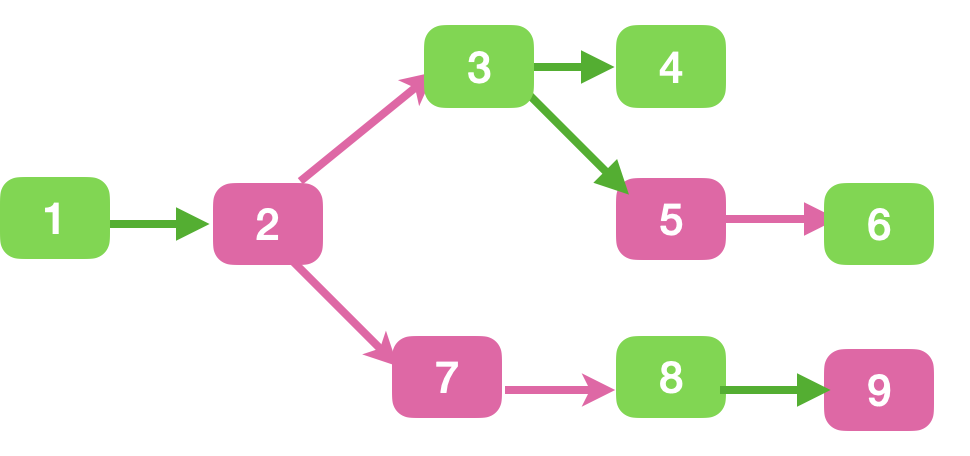
\includegraphics[width=\linewidth]{diagrams/heap.png}
} 
&
\resizebox{5cm}{!}{
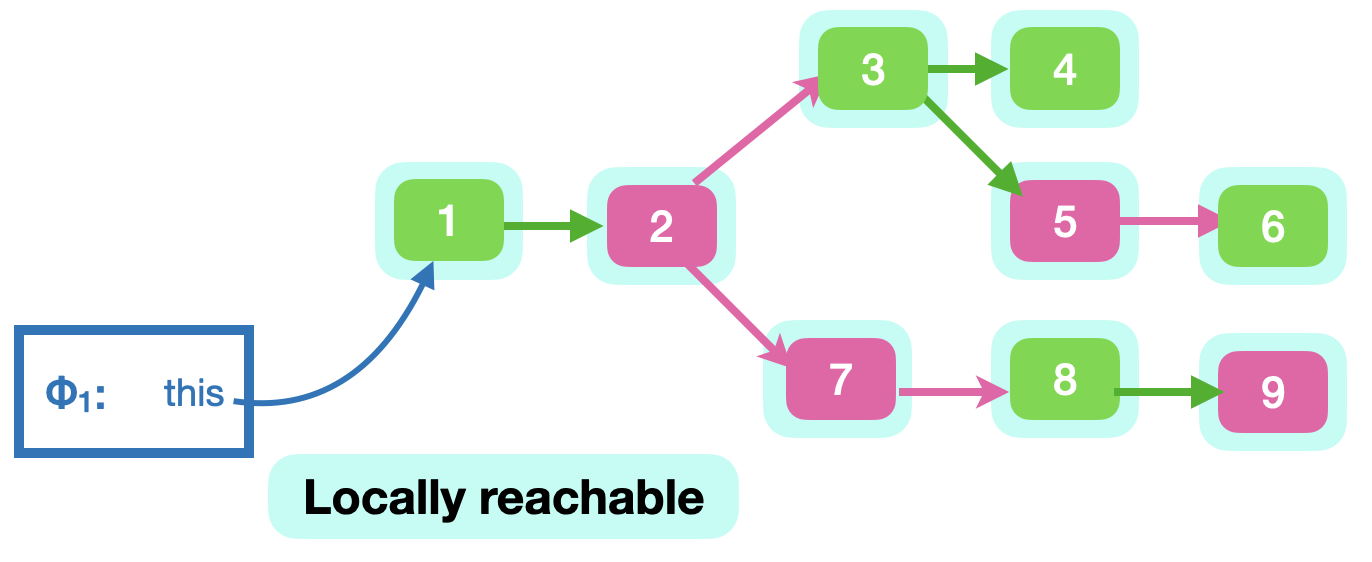
\includegraphics[width=\linewidth]{diagrams/locReachA.png}
} 
&
\resizebox{5cm}{!}{
\includegraphics[width=\linewidth]{diagrams//locReachb.png}
} 
\\
\hline
 a heap
&
Locally Reachable from $\phi_1$
&
Locally Reachable from $\phi_2$
\\
\hline \hline
\end{tabular}
   \caption{A heap, two stacks, and Locally Reachable Objects.
  Distinction  objects into  green/pink  explained later. } % from $\phi_1$ and $\phi_2$. } % n later chapters}
   \label{fig:LReachable}
 \end{figure}

We illustrate these concepts in Fig. \ref{fig:LReachable}:  In the middle pane the top frame is $\phi_1$ which maps \prg{this} to $o_1$; all objects are locally reachable. 
In the right pane the top frame is $\phi_2$, which maps \prg{this} to $o_3$, and $x$ to $o_7$; now $o_1$ and $o_2$ are no longer locally reachable.

Lemma  \ref{lemma:relevant} % describes properties of global reachability. 
says that 
(\ref{oneLR}) any object which is locally reachable after pushing a frame was locally reachable before pushing that frame, and 
(\ref{threeLR}) a pre-existing object, locally reachable after any number of scoped execution steps, was locally reachable at the first step.
\footnoteSD{cite ``only connectivity begets connectivity''}

\begin{lemma}
\label{lemma:relevant}
\label{lemma:push:N}
For all modules $\Mtwo$, states $\sigma$, $\sigma'$,   and frame $\phi$:
\begin{enumerate}
\item
\label{oneLR}
\sdN{$ \sigma'= \PushS {\phi} {\sigma}   \ \wedge  \  {Rng(\phi)} \subseteq \LRelevantO  {\sigma} 
 \ \  \Longrightarrow\ \ \LRelevantO {\sigma'}\  \subseteq \LRelevantO   {\sigma}$}
\item
\label{threeLR}
\sdN{${\leadstoBoundedStar {\Mtwo}  {\sigma}    {\sigma'}}  \ \  \Longrightarrow\ \ 
dom(\sigma) \cap \LRelevantO {\sigma'} \subseteq   \LRelevantO {\sigma}$
}

\end{enumerate}
\end{lemma}

{Consider Fig.  \ref{fig:UpSemantics}. %, and Fig.  \ref{fig:UpSemanticsBounded}.
Lemma \ref{lemma:relevant}, part \ref{threeLR}  promises that any objects locally reachable in $\sigma_{14}$ which already existed in $\sigma_{8}$, were locally reachable in $\sigma_{8}$. However, the lemma is only  applicable to scoped execution, and as 
$\notLeadstoBoundedStar {\Mtwo} {\sigma_8}  {\sigma_{17}}$, 
the lemma does not promise that  objects locally reachable in $\sigma_{17}$ which already existed in $\sigma_{8}$, were locally accessible in $\sigma_{8}$ -- namely it could be that objects are made globally reachable upon method return, during the step from $\sigma_{14}$ to $\sigma_{15}$.}

 
  
  
  
%\footnote{A stronger lemma can be proven:
%% Lemma \ref{lemma:push:N:S} says that % $\pushSymbol$ characterizes  calls and returns. 
%\  (\ref{pushOne}):\  If $\leadstoOrig {\Mtwo} {\sigma}   {\sigma'} $ and $\sigma'\!\in\!\PushS   {\alpha} {\sigma}$ then $\sigma'$ is a  \emph{called} state of $\sigma$ --  {a direct successor state of    $\sigma$  after calling a method}. % with receiver and arguments $\overline \alpha$): \ 
%$\sigma'\in   \PushS  {\alpha} {\sigma}  \ \ \Longleftrightarrow \ \ 
%\exists x, m.[\ \ \sigma.\prg{cont} \txteq x:=y_0.m(y_1,..y_n); \_\ \ \wedge \ \overline \alpha = \overline{ \interpret \sigma y} \ \ ] $
%\\
% (\ref{pushTwo}):\  If $\leadstoOrig {\Mtwo} {\sigma}   {\sigma'} $ and $\sigma\! \in\! \PushS   {\alpha} {\sigma'}$  then $\sigma'$ is a  \emph{caller} state  of $\sigma$ -- {a direct successor  of $\sigma$}  after returning from a method:
% \ \ 
% $\sigma\in   \PushS  {\alpha} {\sigma'}  \ \ \Longleftrightarrow \ \ \exists x, \alpha'.[\ \  \sigma.\prg{cont}\txteq\alpha' \ \ \wedge \ \ \sigma'.\prg{cont}\txteq x:=\alpha';\_ \ \ ] $
% }
  

